%GD can be used in many scenarios such as multi-task learning, semi-supervised learning, and reinforcement learning. 
As generalized distillation only requires the training inputs $\{x_i,y_i\}_{i=1}^n$ and the output $s_i$ from the teacher function $f^{(t)}$, it can be naturally applied to SDA. This leads to \textit{Generalized Distillation Semi-supervised Domain Adaptation} (\textbf{GDSDA}), where the source model can be used as the teacher to output the soft labels and the student model is the target model. To be consistent with other works in domain adaptation, we use source model and target model to denote the teacher model and the student model in the rest of our paper.

An important issue of applying GD to SDA is that, in Eq. \eqref{eq:distill}, each example is assigned with a hard label $y$ (true label) and a soft label $s$ (class probabilities from the teacher). However, in SDA, we are not able to obtain the hard labels of the unlabeled data. Here we follow the GD work\cite{lopez2015unifying} and use the "fake label" strategy to label the unlabeled data: for the labeled examples, we use \textit{one-hot} strategy to encode their labels while using the \textit{gray code} (all 0s) as the label of the unlabeled examples. Thus, each example in the target domain is assigned with a label. It is arguable that the "fake label" strategy would introduce extra noise and degrade the performance. However, we will show in our experiment that this noise can be well controlled by setting a proper value to the imitation parameter and we can still achieve improved performance (See the single source experiment).
\begin{figure}
	\centering
	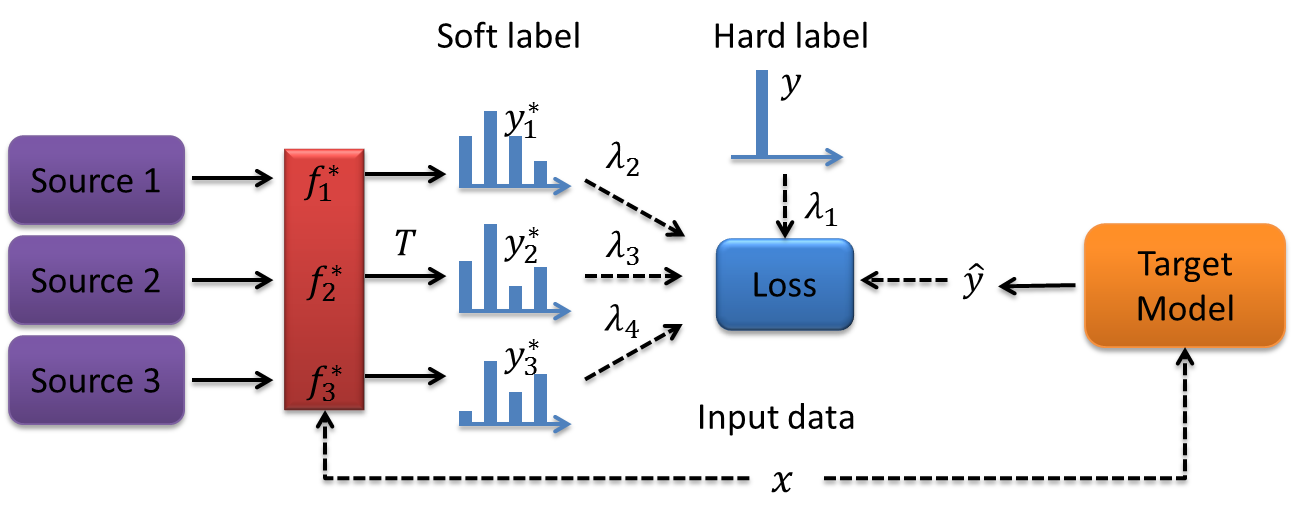
\includegraphics[scale=.4]{figure/multi-GDDA.png}
	\caption{Illustration of GDSDA training process.}
	\label{fig:GDSDA}
\end{figure}
The process of GDSDA is shown in Figure \ref{fig:GDSDA}. Suppose we have $M-1$ source domains denoted as $D_s^{(j)}=\{X^{(j)},Y^{(j)}\}_{j=1}^{M-1}$ and the target domain $D_t=\{X,Y\}$ encoded with the "fake label" strategy. Similar to GD, the process of GDSDA is as follows:
\begin{enumerate}
    \item Train the source models $f^*_j$ for each of the $M-1$ domain with $\{X^{(j)},Y^{(j)}\}$.
    \item For each of the training example $x_i$ in the target domain, computer the corresponding soft label $y^*_{ij}$ with each of the source model $f^*_j$ and the temperature $T>0$.
    \item Learn the target model $f_t$ using the $(M+1)$-tuples $\{x_i,y_i,y^*_{i1},\dots,y^*_{i(M-1)}\}_{i=1}^L$ with the imitation parameters $\{\lambda_i\}^M_{i=1}$ using \eqref{eq:GDDA_abs}:
\end{enumerate} 
\begin{equation}\label{eq:GDDA_abs}
\begin{aligned}
f_t(\lambda)=\underset{f_t \in \mathcal{F}}{\arg \min}&\frac{1}{L}\sum_{i=1}^{L}\bigg[\lambda_1\ell\left(y_i,f_t(x_i)\right)+\sum_{j=1}^{M-1}\lambda_{j+1}\ell\left(y^*_{ij},f_t(x_i)\right)\bigg]\qquad\\
 &\text{s.t.} \qquad \sum_i\lambda_i=1
\end{aligned}
\end{equation}
Compared to other works of SDA which require to use each example of the source domain, by either re-weighting \cite{Donahue_2013_CVPR,duan2012visual} or augmentation \cite{daume2010frustratingly}, GDSDA only requires the trained model from the source domain to generate the soft labels. 
%Considering the fact that it is more convenient to access the source model than each of the examples of the source domain, GDSDA can be more useful than those previous methods. For example, if we want to use ImageNet \cite{imagenet_cvpr09} as the source domain, it is almost impossible to access each of the millions of the examples while there are many well trained models publicly available online that can be used for GDSDA. 
Moreover, GDSDA is able to handle the multi-class scenario while some previous works, such as SHFA\cite{duan2012learning} can only solve the binary classification problem in SSDA. Moreover, GDSDA is compatible with any type of source model that is able to output the soft label (i.e. class probabilities).

\subsection{Why does GDSDA work}
In this part, we provide demonstrate the scenarios where GDSDA would work. Before we provide our analysis, we first introduce the two basic assumptions for GDSDA to work well in domain adaptation: the \textit{assumption of distillation and the assumption of the source model}.

\textbf{Assumption of Distillation:} The capacity (or VC dimension) of the target model $f_t$ is smaller than the capacity of source model $f^*$. This assumption is inherited from distillation.
\textbf{Assumption of the source model:} The source model $f^*$ should work better than a target model $f'_t$ trained only with the hard labels. For example, when we only have a single labeled example for each class in the target training set, it is reasonable to assume that the source model trained from another domain could perform better than any model trained only with the target training data on the target task. Based on this two assumptions, we will show that GDSDA can effectively leverage the source model and transfer the knowledge between different domains under the SDA setting.

According to ERM principle\cite{vapnik1999overview}, the simple model has better generalization ability than the complex one if they both have the same training error.
By mimicking the output of the source model $f^*$ on the target domain, the target model $f_t$ can achieve similar training error to the training error of the source model $f^*$ on the target domain and we can expect that the target model has better generalization ability.
%Previous work \cite{hinton2015distilling} suggests that if the target model can simulate the outputs of the source model, i.e. the soft label, well enough on the training data, the target model could outperform the source model on this task. 

It is worthy to notice that in this process, the target model only has to mimick the output of the source model (soft label) without considering the hard labels of the examples. In another word, GDSDA provide an effective way to utilize the unlabeled data.

Arguably, because of the domain shift, the source model is biased towards the source domain when applying on the target task. However, as it is suggested in \cite{hinton2015distilling}, we can use a few labeled data from the target domain to compensate for the domain shift and achieve a better performance on the target task with Eq. \eqref{eq:GDDA_abs}. Specifically, we use the imitation parameter $\lambda$ to control the relative importance of the soft label from the source model and the hard label, which in turn reflects the similarity between the source and target tasks. 
For example, in Figure \ref{fig:GDSDA}, when we set $\lambda_2=0$, we actually ignore the knowledge from source domain 1.
As a result, with proper imitation parameter, GDSDA can compensate for the domain shift under the setting of SDA (for more details, please see the experiment section).

%\subsection{Key parameter: the imitation parameter}\label{sec:key}
As we have mentioned above, the imitation parameter controls the importance of the soft label, i.e. the knowledge transferred from source domain.
Many previous works have addressed the importance of knowledge control in domain adaptation \cite{duan2012learning,duan2012visual}. Without carefully controlling the amount of knowledge transferred from the source domain, it is easy for the target model to get degraded performance or even suffer from negative transfer \cite{pan2010survey}.
How to choose the imitation parameter is essential for GDSDA. In the previous works, the imitation parameter can only be determined by either brute force search \cite{lopez2015unifying} or background knowledge \cite{Tzeng_2015_ICCV}. On the other hand, in real applications, it is common that there could be multiple source domains to be exploited. As it is suggested in \cite{tommasi2014learning}, learning from multiple related sources simultaneously can significantly improve the performance of the target model. However, these previous works become more difficult to apply when there are multiple sources and imitation parameters to be determined.
For these reasons, we proposed a method, GDSDA-SVM that can estimate the transfer parameter automatically.

%In the following, we show that we should choose the imitation parameter that minimizes the empirical risk on the training data for distillation.

%Let $f(x,\lambda)$ be a function with a finite VC dimension $h$ that minimizes the number of errors on the training data $\{x_i,y_i\}_{i=1}^L$. Let $v(\lambda)$ be the training error. Then according to the VC theory \cite{vapnik1999overview}, for an arbitrary loss function $\mathcal{L}(\cdot)$ we have the following bound:
%\begin{equation}\label{eq:lambda_constraint}
%P\left(\mathcal{L}\left(y,f(x,\lambda)\right)\geq 0\right) < v(\lambda)+O\left(\sqrt{\frac{h}{L}}\right)
%\end{equation}
%In other word, the optimal imitation parameter should be the one that can minimize the training error.  

%In the previous work, the imitation parameter can only be determined by either brute force search \cite{lopez2015unifying} or background knowledge \cite{Tzeng_2015_ICCV} which greatly reduces its effectiveness. In domain adaptation, it is common that there could be multiple source models to be exploited. It is ideal to find a method that can determine the imitation parameter automatically.
